\section*{Einleitung}
Die Erfindung des \glqq scanning tunneling microscope\grqq (STM) machte erstmals die atomare Auflösung von Oberflächen möglich.
Das grundlegende Konzept beruht dabei auf der Nutzung des stark abstandsabhängigen Tunnelstroms zwischen der Probe und einer scharfen Spitze.
Eben dieses Funktionsprinzip stellt eine intrinsische Begrenzung des STM dar.
Nur metallische Oberflächen können mit dieser Methode betrachtet werden.
Das \glqq atomic force microscope\grqq (AFM) macht es möglich auch nicht-leitende Materialien aufzulösen, da hierbei die Kraft zwischen Spitze und Probe bei Distanzen von ca. $\SI{1}{nm}$ ausgenutzt wird.
Es bildet die Weiterentwicklung des STM und des stylus profilometers, wessen Auflösung durch die Größe seiner Spitze ($\sim 1\mu m$) begrenzt ist.
Ein weiterer gravierender Vorteil gegenüber dem STM besteht beim AFM darin, dass es auch an der Luft und bei Raumtemperatur bedient werden kann.
Vor diesem Hintergrund wurden in diesem Experiment mehrere Proben vermessen, um die Leistungskraft dieses Verfahrens bei der Untersuchung ihrer Topographien aufzuzeigen.

\section{Theorie}
\subsection{Kraft zwischen Spitze und Probe}
    Bei einem Spitzen-Proben Abstand von $> \SI{1}{nm}$ stellen die attraktiven langreichweitigen Kräfte, die unter der Van-der-Waals-Wechselwirkung zusammengefasst werden können, die größte Kraft dar. Diese beruhen jeweils auf der Coulomb-Wechselwirkung.
    \hspace{3cm}
    \begin{description}
        \item[Dipol-Dipol-WW:]  Diese Kraft bildet sich zwischen zwei permanent polaren Molekülen aus, die einander anziehen.
        \item[Induktions-WW:]  Kraft zwischen polarem und neutralem Molekül, wobei das Polare dem Neutralen ein magnetisches Dipolmoment induziert.
        \item[London-Dispersions-WW:]  Diese Kraft wirkt zwischen zwei neutralen Molekülen. Durch Fluktuationen entstehen spontane elektrische Dipole, die sich gegenseitig anziehen.
    \end{description}
    Die letzte überwiegt meist gegenüber den anderen beiden Kräften. \\
    Unter der Annahme zweier Edelgsatome lässt sich ihr Wechselwirkungspotential mit der Abstandsabhängigkeit
    \begin{equation*}
        V_{\mathrm{VdW}(r)} \propto -\frac{1}{r^6}
    \end{equation*}
    ausdrücken.

    Bei einem Spitzen-Proben Abstand von $< \SI{1}{nm}$ entstehen kurzreichweitige WW aufgrund des Überlapps zwischen den elektronischen Zustandsdichten.
    Wird der Abstand in fallender Ordnung durchlaufen, so ist die Wechselwirkung erst attraktiv, da durch den Überlapp der äußeren offenen Schalen chemische Bindungen entstehen, die die Gesamtenergie minimieren. \\
    \setlength{\columnsep}{10pt}
    \begin{wrapfigure}{r}{0.4\textwidth}
        \centering\captionsetup{margin={0.5cm,-1cm}, format=plain}
        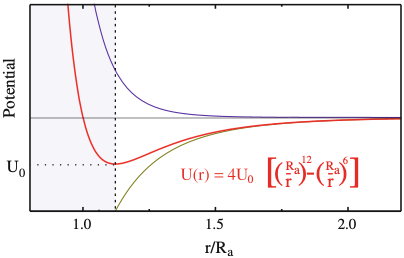
\includegraphics[width=0.48\textwidth]{bilder/Lennard_Jones_Potential.png}
        \caption{Hier ist das Lennard-Jones-Potential, seine zugehörige Kraft und dessen negierte Ableitung dargestellt.}
        \label{fig:Lennard_Jones_Potential}
    \end{wrapfigure}
    Dann kommen sich die Spitze und Probe so nah, dass die geschlossenen Orbitale überlappen.
    Die kernnahen Elektronen müssen aufgrund des Pauli-Verbotes in höhere Zustände ausweichen.
    D.h. sie müssen effektiv weiter vom Kern des anderen, an der Wechselwirkung beteiligten, Atoms entfernt sein.
    Diese Wechselwirkung wird durch
    \begin{equation*}
        V_{\mathrm{Pauli}(r)} \propto \frac{1}{r^{12}}
    \end{equation*}
    beschrieben.
    Die gesamte Wechselwirkung zwischen Sptize und Probe lässt sich also in erster Näherung durch das Lennard-Jones-Potential
    \begin{equation*}
        U(r) = 4 U_0 \left[\left(\frac{R_a}{r}\right)^{12} - \left(\frac{R_a}{r}\right)^6\right]
    \end{equation*}
    schreiben, wobei $U_0$ die Tiefe des Potentialminimums ist und $R_a$ der Abstand ist, bei dem $V(r) = 0$ gilt.
    Im obersten Graphen in \autoref{fig:Lennard_Jones_Potential} ist das Potential mit den soeben beschriebenen Parametern zu erkennen.
    Die gestrichelte Linie grenzt den repulsiven von dem attraktiven Effekt der Wechselwirkung ab.

    Eine weitere Kraft, die bei der Wechselwirkung zwischen Spitze und Probe eine große Rolle spielt, ist die elektrostatische Wechselwirkung.
    Sie entsteht durch unterschiedliche Austrittsarbeiten bzw. durch eine Ladung auf der Spitze und Probe, sodass .


\subsection{Cantilever und Spitze}

\subsection{Piezo}

\subsection{Detektion}

\subsection{Messmodi}


% \begin{figure}[ht]
%     \centering
%     \includegraphics[width=0.8\textwidth]{bilder/emission.jpg}
%     \caption{The absorption and emission processes in the active medium are shown for a two state system. \cite{anleitungHeNe}}
%     \label{fig:emission}
% \end{figure}


% \begin{figure}
%     \centering
%     \begin{subfigure}{0.49\textwidth}
%         \includegraphics[width = \textwidth]{bilder/n_Donatorschema_demtroeder.png}
%         \caption{n-doped}
%     \end{subfigure}
%     \hfill
%     \begin{subfigure}{0.49\textwidth}
%         \includegraphics[width = \textwidth]{bilder/p_Donatorschema_demtroeder.png}
%         \caption{p-doped}
%     \end{subfigure}
%     \caption{The Band structures with the fermi energy and the donor and acceptor states sre shown for p- and n-doped materials \cite{demtroeder}}
%     \label{fig:doting}
% \end{figure}
